\documentclass{article}
\usepackage{graphicx, float, url, hyperref, afterpage, amsthm, amsmath, multirow}

\title{Comparison of Boosted Perceptrons and Support Vector Machines}
\author{Joshua Frankie Rayo\\2011-19612\\CS 280 Programming Assignment 3}
\date{\today}

\begin{document}

\maketitle
\tableofcontents

\section{Introduction}
	In this paper the performance of boosted perceptrons are compared against support vector machines. Performance measures of these classifiers include accuracy rate, training time and testing time. The former classifier are actually an ensemble of perceptrons that is trained using the adaptive boosting algorithm its individual performance. This is implemented using Python that makes computations in vector form and as easy as possible. A third-party library LibSVM is used to instantiate the support vector machines.
\section{Methodology}
The classifier is made using Python, a high level, general-purpose programming language that is relatively easy to learn and has very good features in list manipulation. Third-party libraries used are \texttt{numpy}, \texttt{matplotlib} and \texttt{libsvm}.
\subsection{Creating the dummy dataset}
The dummy dataset is easily formed using the function \texttt{numpy.random.multivariate\_normal} that generates random points given the mean and covariance of a multivariate normal distribution. For the negative class, 100 points are randomly generated with mean $\mathbf{\mu_1} = (0,0)$ and variance $\mathbf{I_2}$. For the positive class, 100 points are randomly generated with mean $\mathbf{\mu_2} = (10,10)$ and variance $\mathbf{I_2}$. Each of the classes are divided into two for training and testing the classifiers.

The dummy dataset can be used primarily to test the classification accuracy of a single perceptron. Unknown vectors which are near $\mathbf{\mu_1}$ using the Euclidean distance should have a negative class and vectors near $\mathbf{\mu_2}$ should be assigned to the positive class.

\subsection{The Splice and Banana Datasets}
From the \texttt{banana} dataset, first 400 points are used in training and remaining 4900 points are used in testing. For the \texttt{splice} dataset, first 1000 training points and remaining 2175 test points are used.

\subsection{The Perceptron}
A Python class is created to simulate the perceptron classifier with a \textit{maxitercnt} attribute that limits the iterations for the pocket (learning) algorithm. In training the classifer, function \texttt{classify($\mathbf{X}, \mathbf{y}$)}, the bias is included in the weight vector $\mathbf{w}$. Consequently the input vector should also be extended into another dimension by adding 1 as its first element so that the $y=\mathbf{w}\cdot\mathbf{x}$ still holds. The function \texttt{predict($\mathbf{X}, \mathbf{y}$)} returns accuracy of a perception instance given a test set, while the function \texttt{outputv($\mathbf{X}$)} assigns an unknown input to its class using the trained weight vector.

\subsection{The Boosted Perceptron}
Another Python class \texttt{Adaboost} is created to simulate the boosted perceptron with attribute $K$ as the number of classifier instances (inducers). This class is composed of many perceptron instances in an object-oriented paradigm. Function \texttt{adabtrain($\mathbf{X}, \mathbf{y}$)} trains the model with $K$ inducers using the adaptive boosting algorithm. The function \texttt{adabpredict($\mathbf{X}, \mathbf{y}$)} returns accuracy of the boosted perceptron given a test set, while the function \texttt{adaboutputv($\mathbf{X}$)} assigns an unknown input to its class using the weighted hypotheses of the inducers.

\section{Results}
\subsection{Boosted Perceptron Population Accuracy}
Initially, 1000 inducers are trained for this classifier. The plot below shows the classifier accuracy when first $K$ inducers are used for computing the outputs.

\begin{figure}[H]
	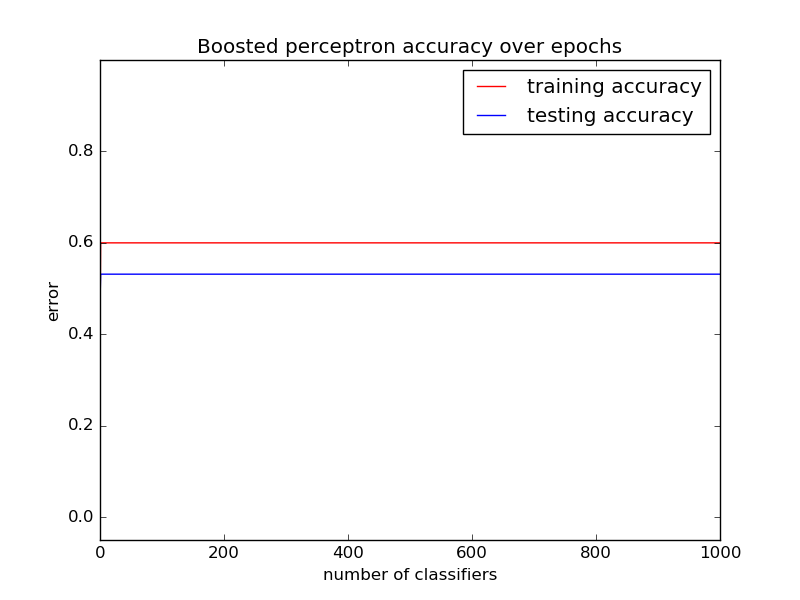
\includegraphics[width=\textwidth]{splice}
	\caption{For the splice dataset, training and testing accuracy (60\%, 52\% respectively) remains constant given an arbitrary number of inducers. This is indeed a remarkable dataset for this classifier.}
\end{figure}

\begin{figure}[H]
	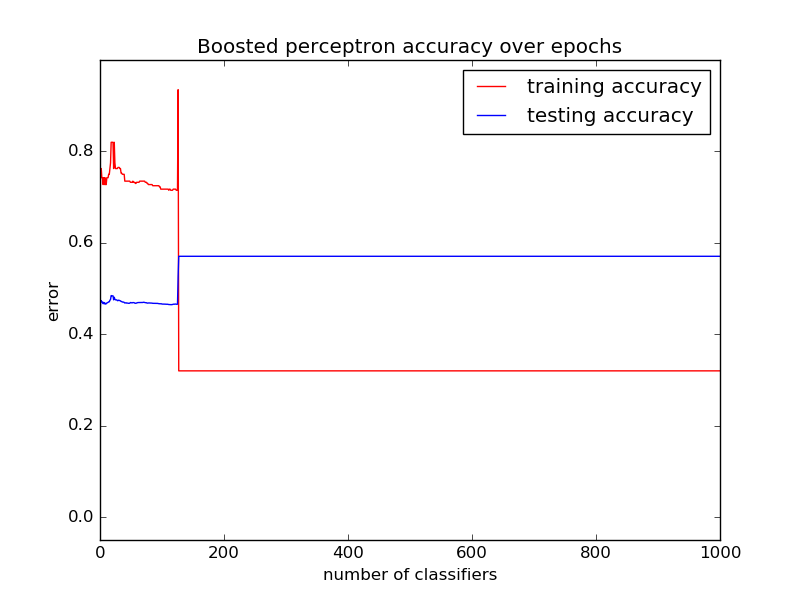
\includegraphics[width=\textwidth]{banana}
	\caption{For the banana dataset, overfitting occurs when $K>126$. It is recommended to use $K=126$ since it makes training and testing accuracy high, 95\% and 58\% respectively.}
\end{figure}

\subsection{SVM Kernel and Parameter Settings}
In training this classifier, one-class SVM \texttt{(-s 2)} is used since there are only two classes to be considered and different kernel function have been used, listed below:
\begin{itemize}
	\item linear \texttt{(-t 0)}
	\item polynomial \texttt{(-t 1)}
	\item radial basis function (RBF) \texttt{(-t 2)}
	\item sigmoid \texttt{(-t 3)}
\end{itemize}

The table below lists the testing accuracy of SVM based on each kernel function with default coefficients and gamma values:

\begin{table}[H]
	\centering
	\begin{tabular}{c | c | c}
		\textbf{kernel/dataset} & \textbf{splice} & \textbf{banana}\\
		\hline
		linear & 56.2759 & 57.0612\\
		polynomial & 56.3218 & 57.0612\\
		RBF & 59.9080 & 57.2245 \\
		sigmoid & 56.4138 & 57.0612
	\end{tabular}
\end{table}

The RBF clearly bested the other kernel functions on both datasets. Moreover, the figures below show the linear and RBF decision curves for the banana dataset, found on \hyperlink{https://www.quora.com/Is-is-true-that-once-we-have-large-data-sets-ML-classifier-selection-does-not-have-much-of-an-effect-What-does-large-mean-here}{Quora}.

\begin{figure}[H]
	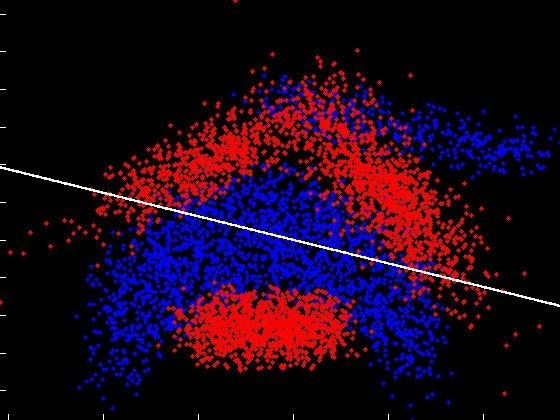
\includegraphics[width=.5\textwidth]{linearbanana}
	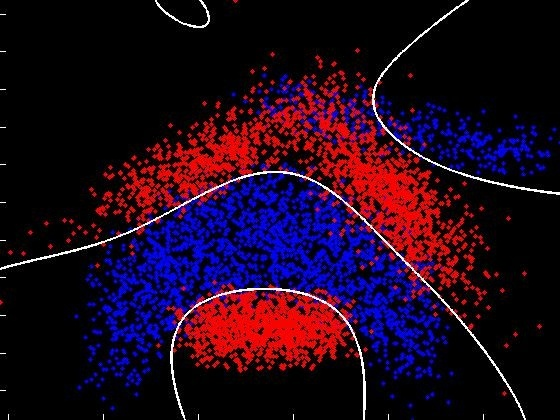
\includegraphics[width=.5\textwidth]{rbfbanana}
\end{figure}

Clearly the decision curve from RBF kernel classifies the banana dataset better than the linear kernel. Its parameter is kept to its default value $\gamma = 1/\text{no\_of\_features}$.

\subsection{Comparison of SVM and Boosted Perceptron}
The accuracy rate and running time of classifiers are the performance measures taken into account. Using the best parameters for SVM and boosted perceptron, the table below shows the performance of each classifier over the \texttt{splice} and \texttt{banana} datasets:

\begin{table}[H]
	\centering
	\begin{tabular}{c | c | c | c}
		\textbf{classifier} & \textbf{dataset} & \textbf{testing accuracy} & \textbf{running time} \\
		\hline
		boosted perceptron & splice & 52 & ~3hrs\\
		$K=126$ & banana & 58 & ~1hr\\
		\hline
		SVM & splice & 59.9080 & 0.8374 s\\
		RBF kernel & banana & 57.2245 & 0.2671 s\\
	\end{tabular}
\end{table}

The results clearly show that support vector machines are still better than boosted perceptrons in terms of accuracy and running time.

\section{Conclusion}
Using the support vector machines generally take much less time in training and testing compared to using ensemble of classifiers that involves traning large number of inducers. It is good to use SVM because of its inherent optimizing property. But if we can only use weak classifiers such as a perceptron, making an ensemble is a very good approach to make a better classifier than their individual perfomances.

\end{document}